\documentclass{beamer}
\usepackage{luatexja}
\renewcommand{\kanjifamilydefault}{\gtdefault}
\usetheme{Copenhagen}
\usepackage{graphicx}
\usepackage{here}

\title{レオンハルト・オイラーについて}
\author{山田 太郎}
\date{\today}


\begin{document}
\begin{frame}
\titlepage
\end{frame}

\begin{frame}\frametitle{レオンハルト・オイラー}
この文書では、18世紀を代表する数学者\textbf{レオンハルト・オイラー}について語ります。

\textbf{レオンハルト・オイラー (Leonhard Euler) }は、1707年にスイスのバーゼルに生まれ、のちの19世紀に続く数学、さらには物理学における膨大な業績を残しました。図\ref{fig:euler}は、オイラーの有名な肖像画です。\pause

\begin{figure}[H]
\centering
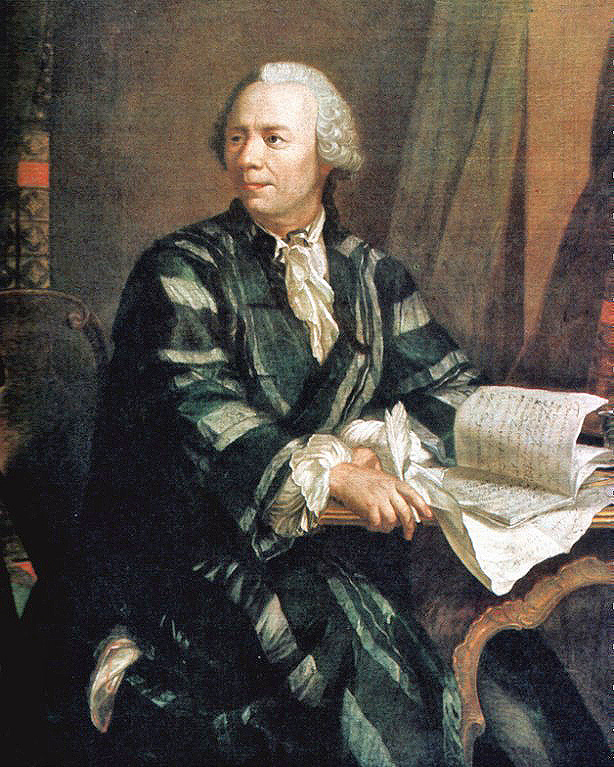
\includegraphics[scale = 0.3]{euler.jpeg}
\caption{レオンハルト・オイラー}
\label{fig:euler}
\end{figure}
\end{frame}

\begin{frame}\frametitle{オイラーの公式}
なんといっても、式(\ref{eq:euler})は、オイラーの業績の中でも特に有名な\textbf{オイラーの公式}です。\pause

\begin{block}{オイラーの公式}
\begin{equation}
e^{ix} = \cos{x} + i\sin{x} \label{eq:euler}
\end{equation}
\end{block}

$e$はネイピア数、$i$は虚数単位、$\cos, \sin$は三角関数です。
\end{frame}

\begin{frame}\frametitle{オイラーの公式}

特に式(\ref{eq:euler})において、$x=\pi$とした式(\ref{eq:euler2})は、虚数単位と円周率、ネイピア数を結び付けるあまりにも美しさゆえに、「宝石のような等式」とまで称されます。\pause

\begin{block}{オイラーの公式 ($x=\pi$) }
\begin{equation}
e^{i\pi}=-1
\label{eq:euler2}
\end{equation}
\end{block}

\end{frame}

\begin{frame}\frametitle{バーゼル問題}

さらに、オイラーの業績の中では、\textbf{バーゼル問題}の解決が有名です。

バーゼル問題とは無限級数の問題の1つで、平方数の逆数すべての和はいくつかという問題ですが、オイラー以前にはベルヌーイという数学者がこの問題を解決するのに失敗しています。バーゼルはオイラーの故郷でもあり、ベルヌーイの故郷でもあるので、バーゼル問題と呼ばれているのですね。\pause

バーゼル問題は、式(\ref{eq:basel})の値がいくらかという問題です。

\begin{block}{バーゼル問題}
\begin{equation}
\sum_{k=1}^{\infty} \frac{1}{k^2} = \frac{1}{1^2} + \frac{1}{2^2} + \frac{1}{3^3} + \cdots + \frac{1}{n^2} + \cdots \label{eq:basel}
\end{equation}
\end{block}
\end{frame}


\begin{frame}\frametitle{バーゼル問題}
レオンハルト・オイラーは、三角関数の無限乗積展開という巧みな手法により、式(\ref{eq:basel})の値が$\frac{\pi^2}{6}$であることを予想し、後にこれが正しい結果であることが証明されました。

バーゼル問題は、リーマンのゼータ関数という素数と密接に関わる関数の特殊値を表しており、その後の数学の発展においても非常に重要な結果を示唆しています。
\end{frame}

\begin{frame}\frametitle{オイラーの生涯}
オイラーは、その類まれなる才能により、語るに余りある数々の業績を残し、その激動の生涯を終えました。表\ref{tab:euler}は、オイラーの生涯をまとめた年表です。\pause

\begin{table}[htbp]
\centering
\caption{オイラーの生涯}
\label{tab:euler}
\begin{tabular}{|l|l|}
\hline
年 & 出来事 \\ \hline \hline
1707年 & スイスのバーゼルに生まれる\\ \hline
1727年 & サンクトペテルブルクの科学学士院に赴任 \\ \hline
1741年 & ベルリン・アカデミーの会員となる \\ \hline
1771年頃 & 両目を失明 \\ \hline
1783年 & 76歳で亡くなる \\ \hline
\end{tabular}
\end{table}
\end{frame}

\begin{frame}\frametitle{オイラーの生涯}
オイラーは、その76年の生涯のうちに人類史上最多といわれるほどの膨大な量の論文や著書を残しました。我々がこうして数学によって支えられた便利な日常生活を送れるのも、オイラーが残した業績のおかげであるところが大きいのです。
\end{frame}
\end{document}

